% Generated by generate_final_paper_figures_CLIPS_CV.m.
% Active main-paper figures

\begin{figure*}[!t]
    \centering
    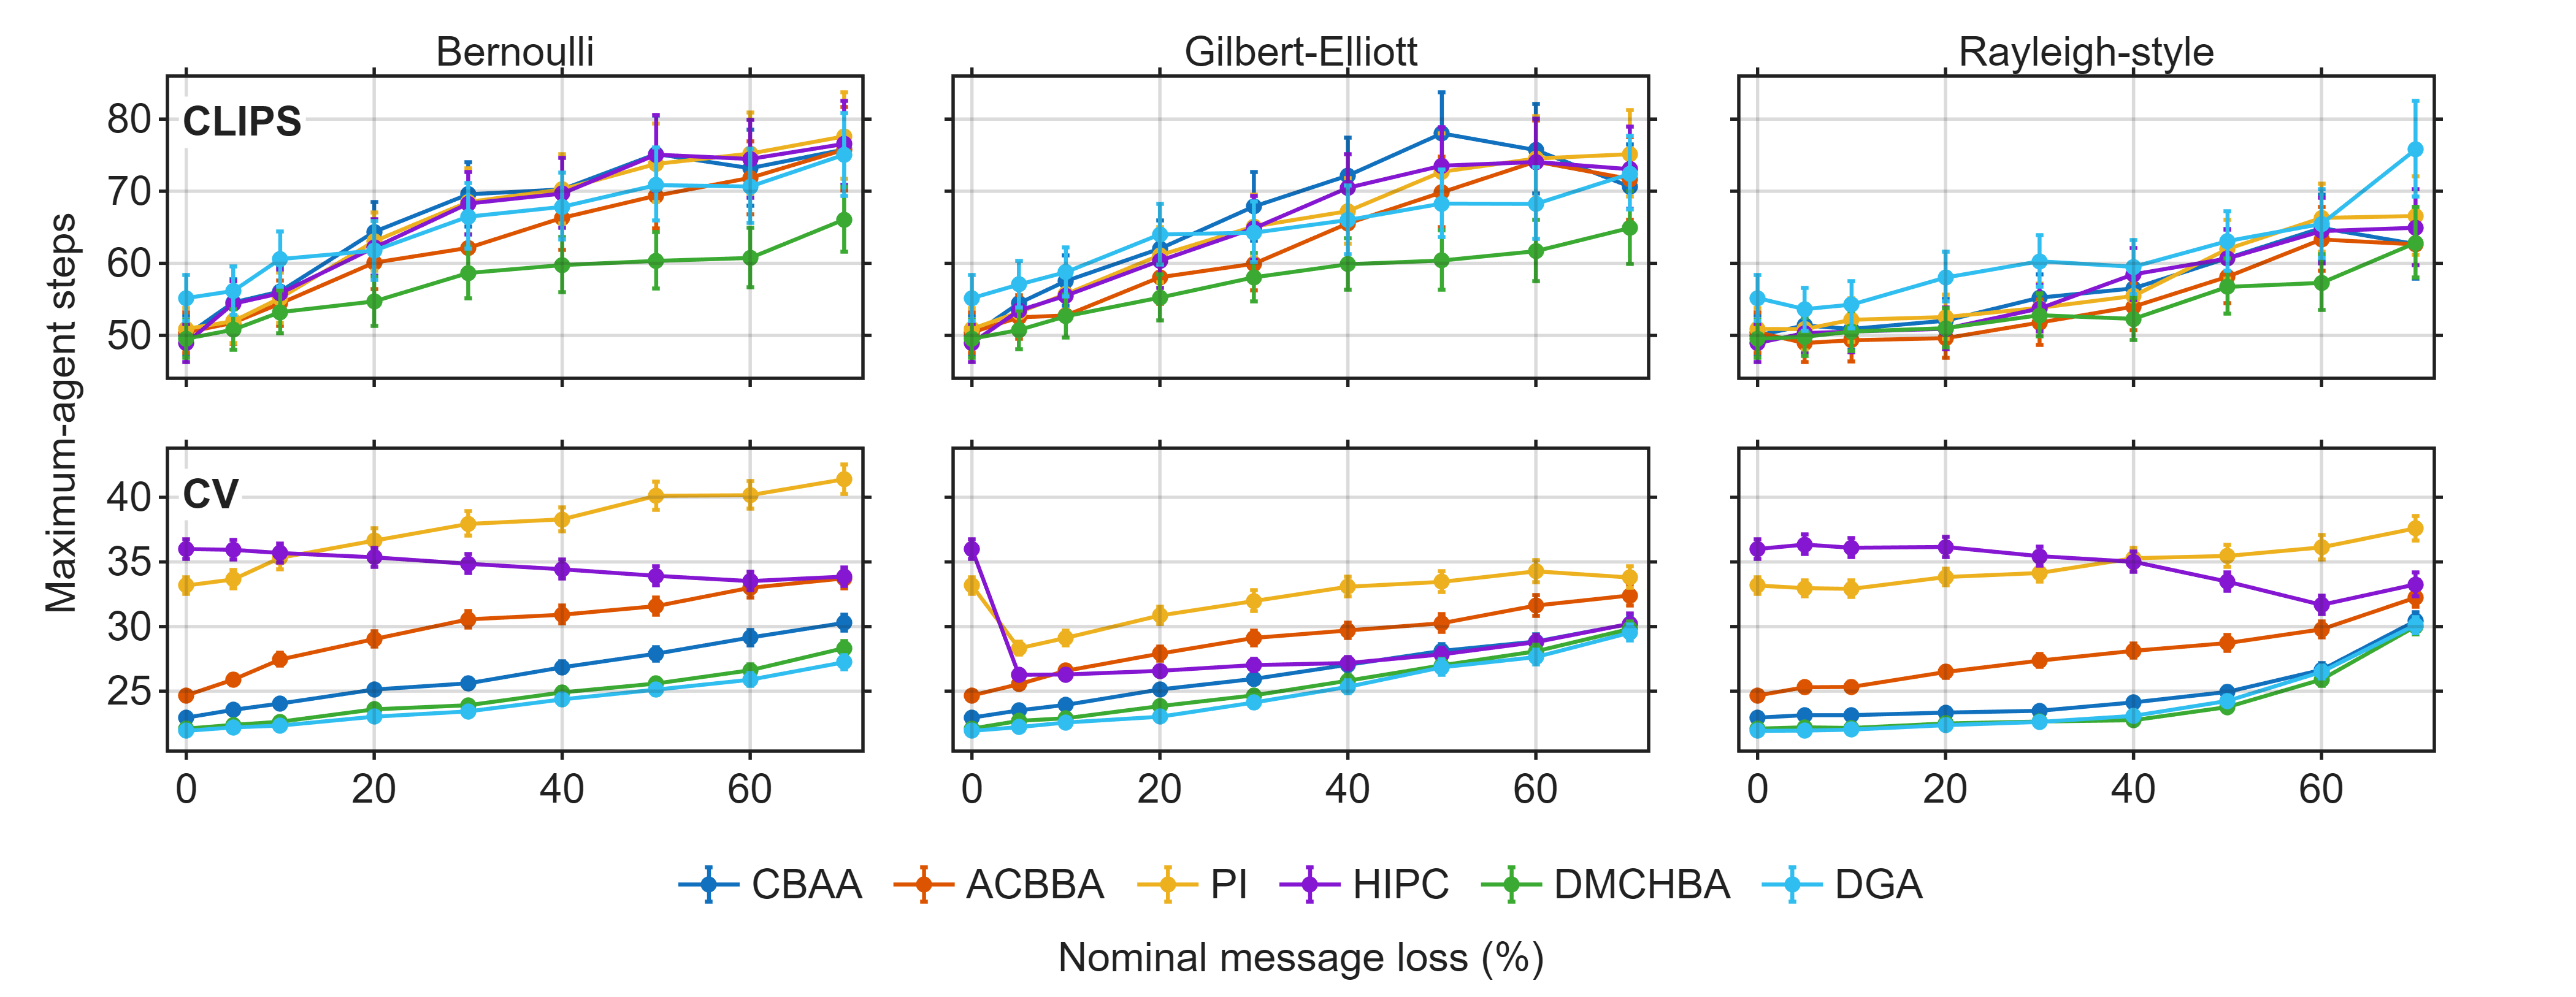
\includegraphics[width=\textwidth]{figures/primary_mission_performance_curves.png}
    \caption{Mission-specific paired performance under Bernoulli, Gilbert--Elliott ($\rho=0.8$), and Rayleigh-style degradation. CLIPS and CV both report maximum-agent steps. Curves show paired means with 95\% confidence intervals.}
    \label{fig:primary_mission_performance}
\end{figure*}

\begin{figure}[!t]
    \centering
    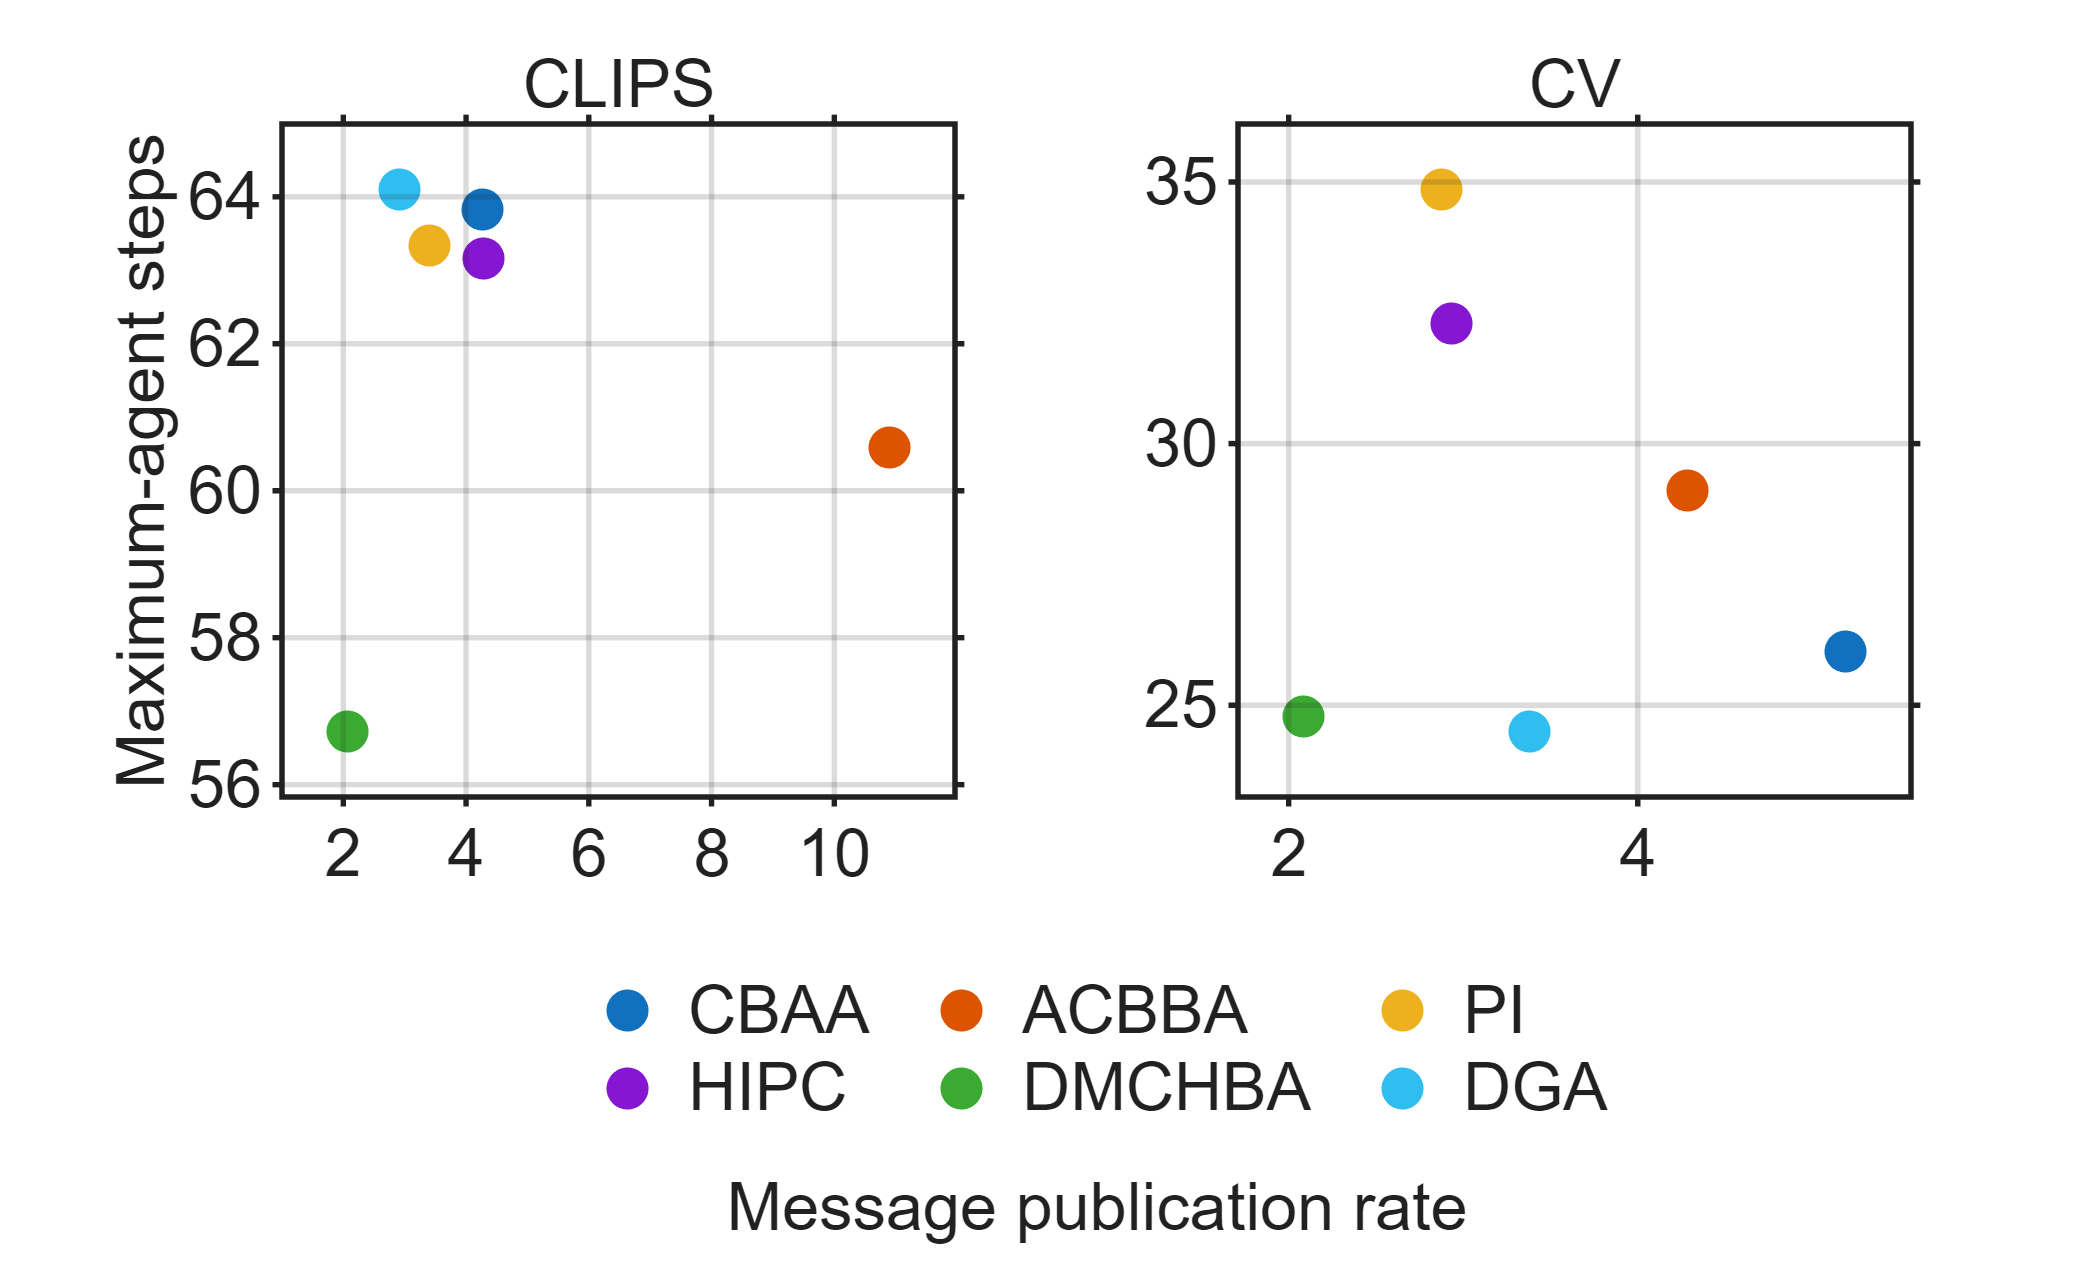
\includegraphics[width=\columnwidth]{figures/communication_performance_tradeoff.png}
    \caption{Communication--performance tradeoff for CLIPS and CV. Each point is an algorithm's unweighted mean across the 24 impaired condition means. The left panel reports CLIPS and the right panel CV. The horizontal axis is message publications per team step and the vertical axis is maximum-agent steps; lower-left is preferable.}
    \label{fig:communication_performance_tradeoff}
\end{figure}
\begin{figure}[!t]
    \centering
    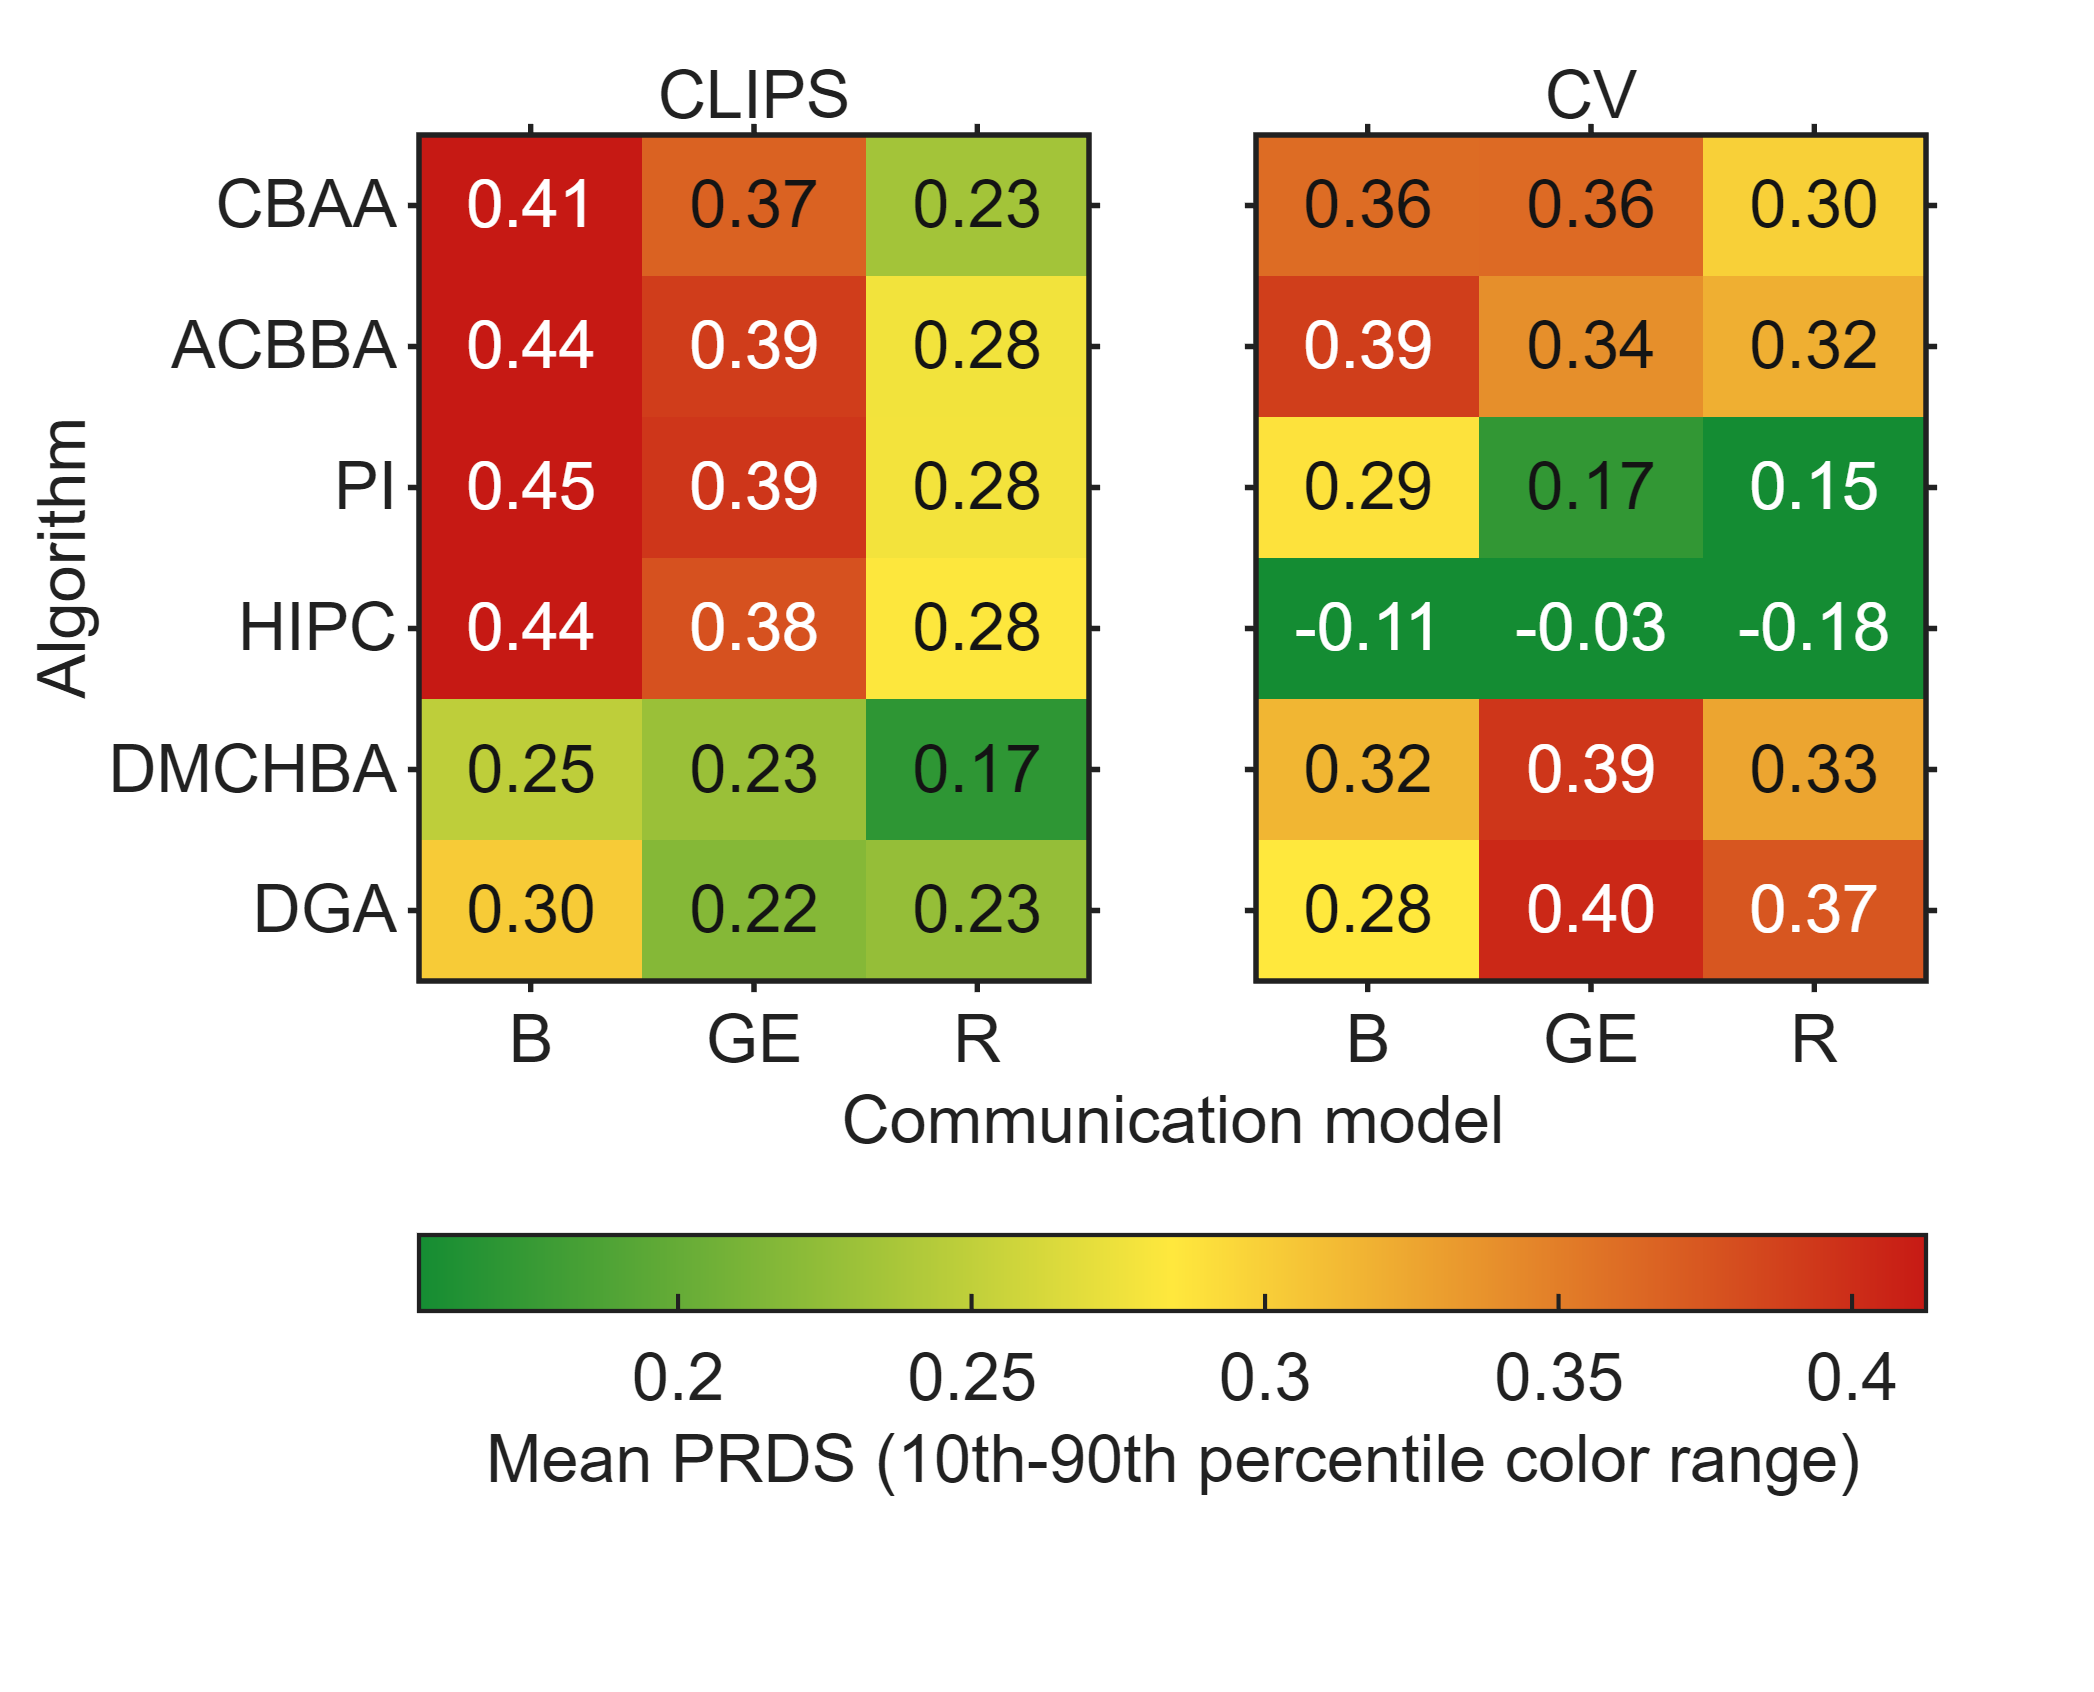
\includegraphics[width=\columnwidth]{figures/prds_supplement.png}
    \caption{Paired relative degradation slope (PRDS) for maximum-agent steps. Columns B, GE, and R denote Bernoulli, Gilbert--Elliott, and Rayleigh-style degradation, respectively. Each cell reports the mean fitted percentage change in $S_{\max}$ per one-percentage-point increase in communication degradation. Within each mission and communication model, all six algorithms use the same complete trial trajectories across ideal communication and all eight degraded levels. Smaller positive values indicate slower degradation from ideal performance, while negative values indicate a decreasing fitted trajectory.}
    \label{fig:prds_supplement}
\end{figure}

\begin{figure}[!t]
    \centering
    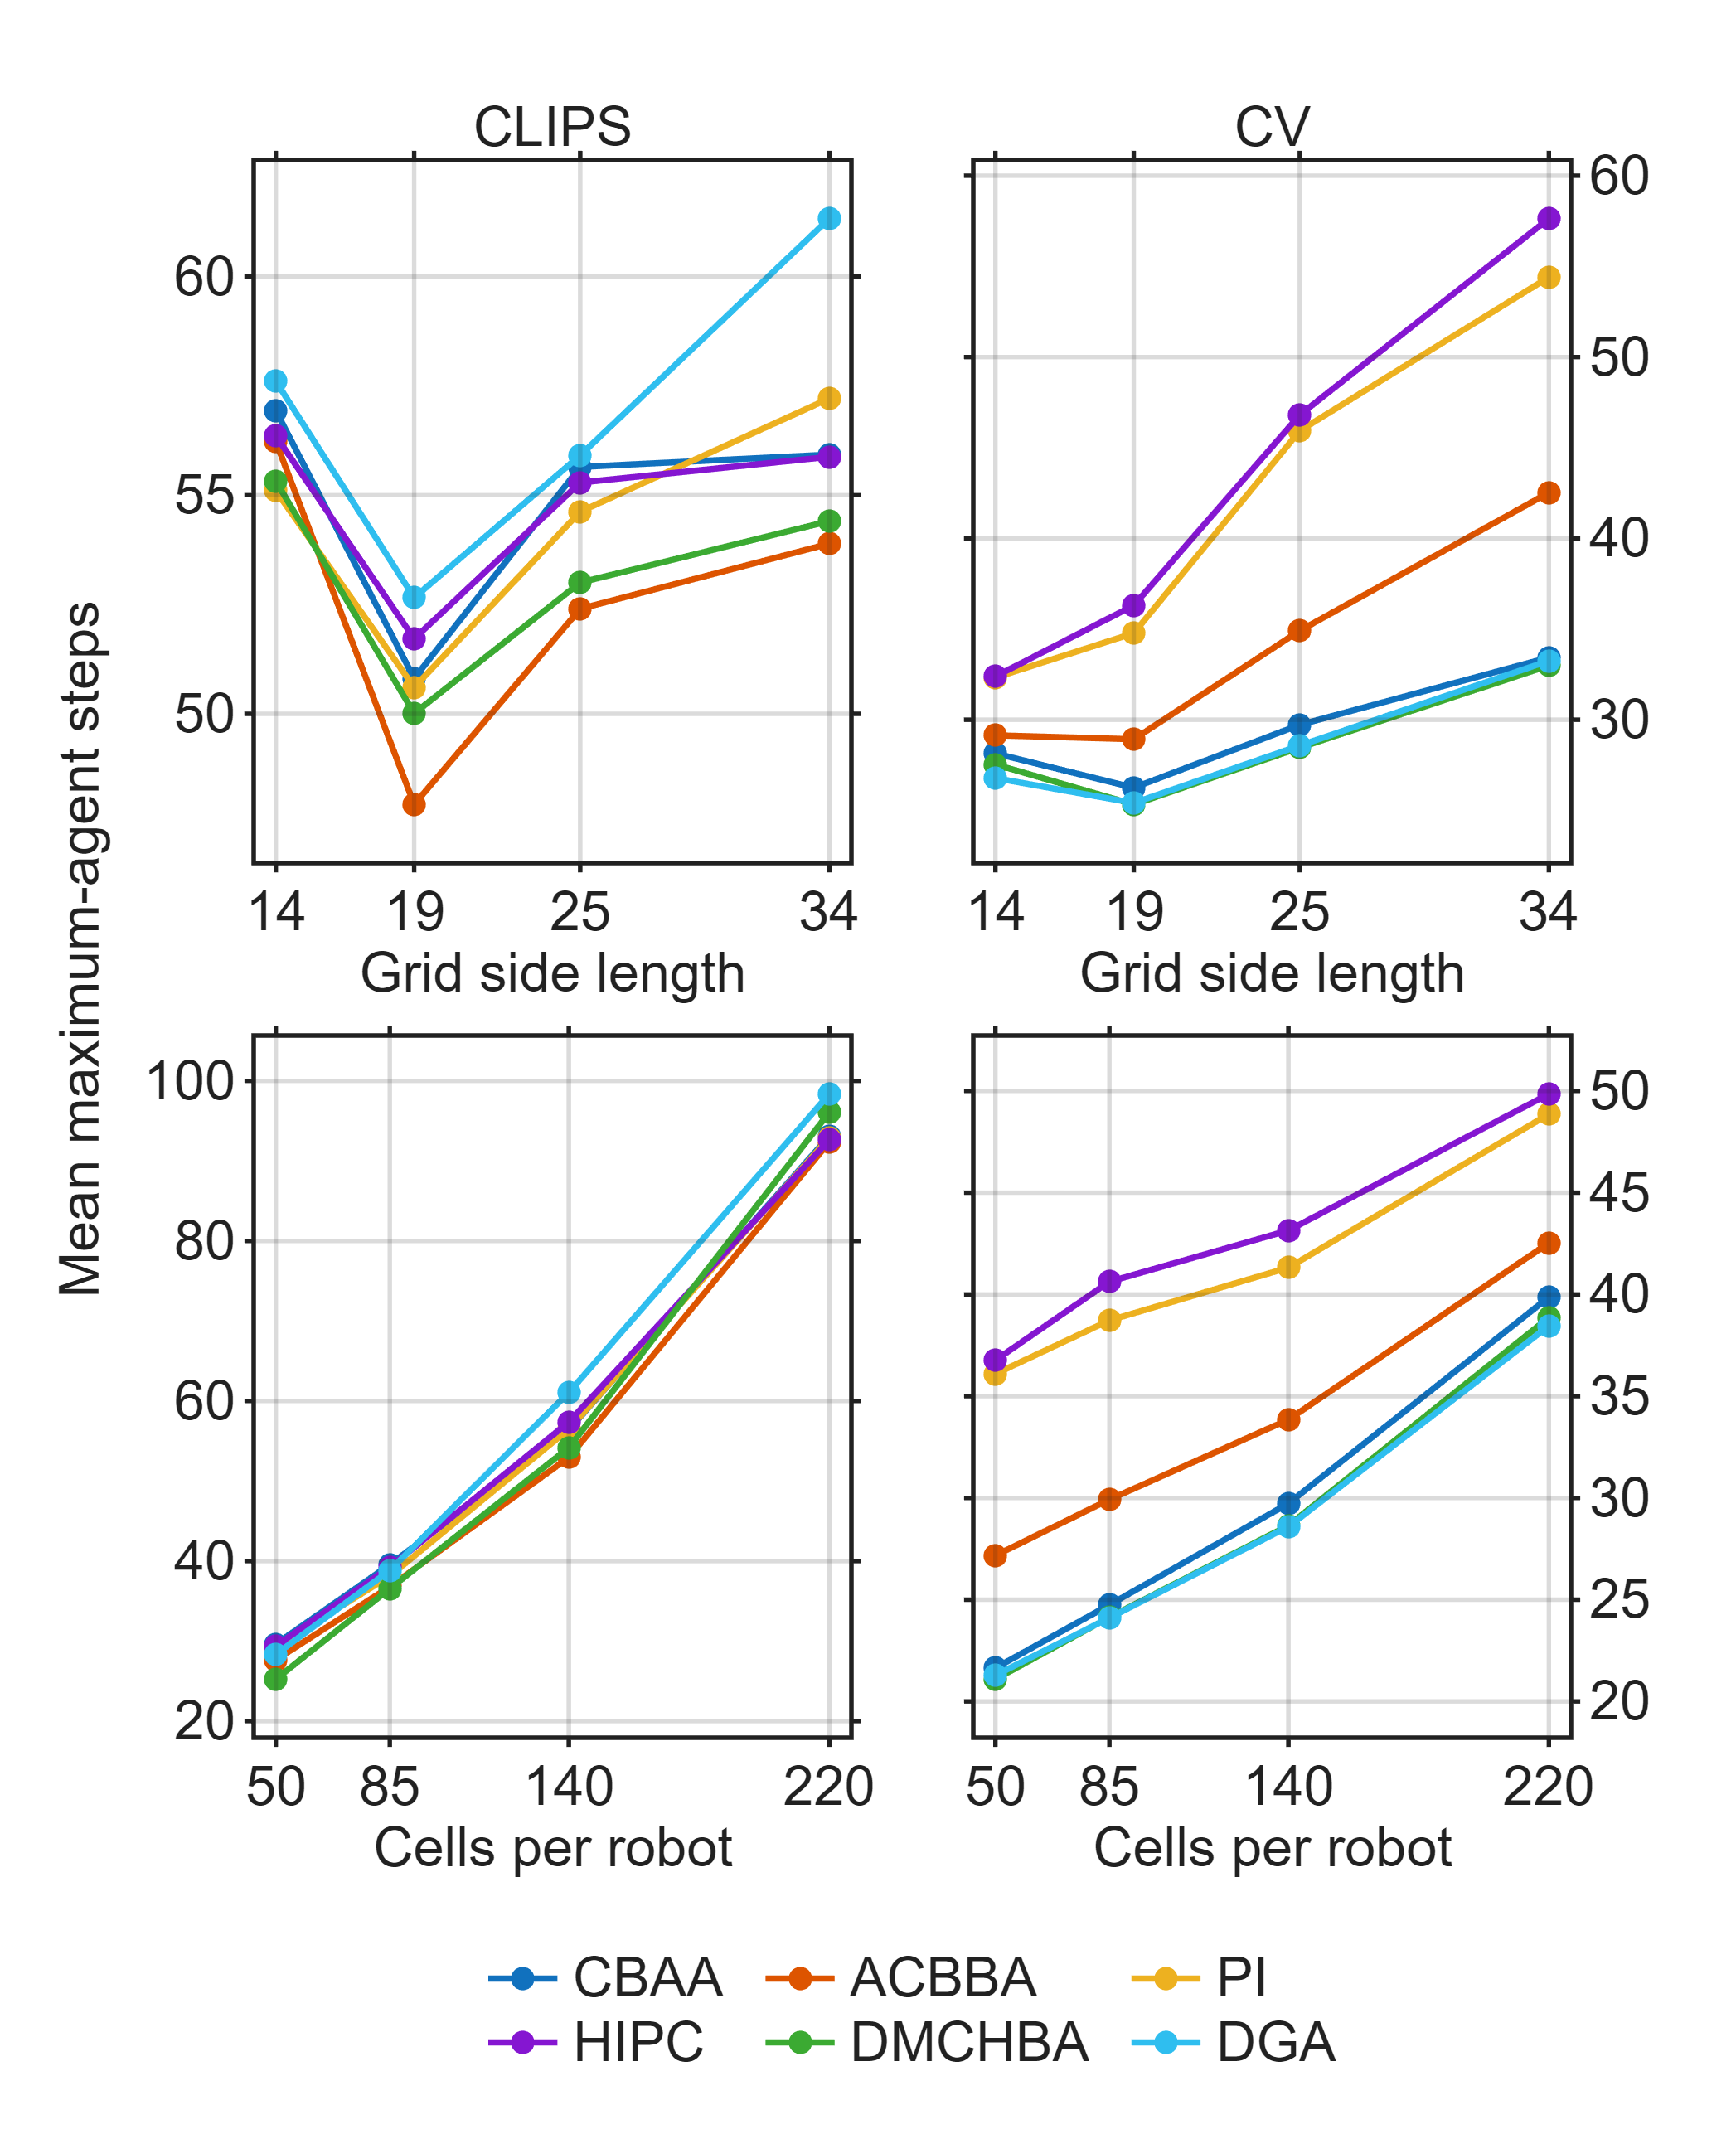
\includegraphics[width=\columnwidth]{figures/grid_density_maximum_agent_steps_summary.png}
    \caption{Maximum-agent-step sensitivity to grid side length and nominal cells per robot. Columns show CLIPS and CV; rows show the two scale factors. Each point pools retained trial blocks across both communication settings and all four opposite-factor levels; a block contributes only when all six algorithms completed with finite maximum-agent steps.}
    \label{fig:grid_density_maximum_agent_steps}
\end{figure}

\begin{figure}[!t]
    \centering
    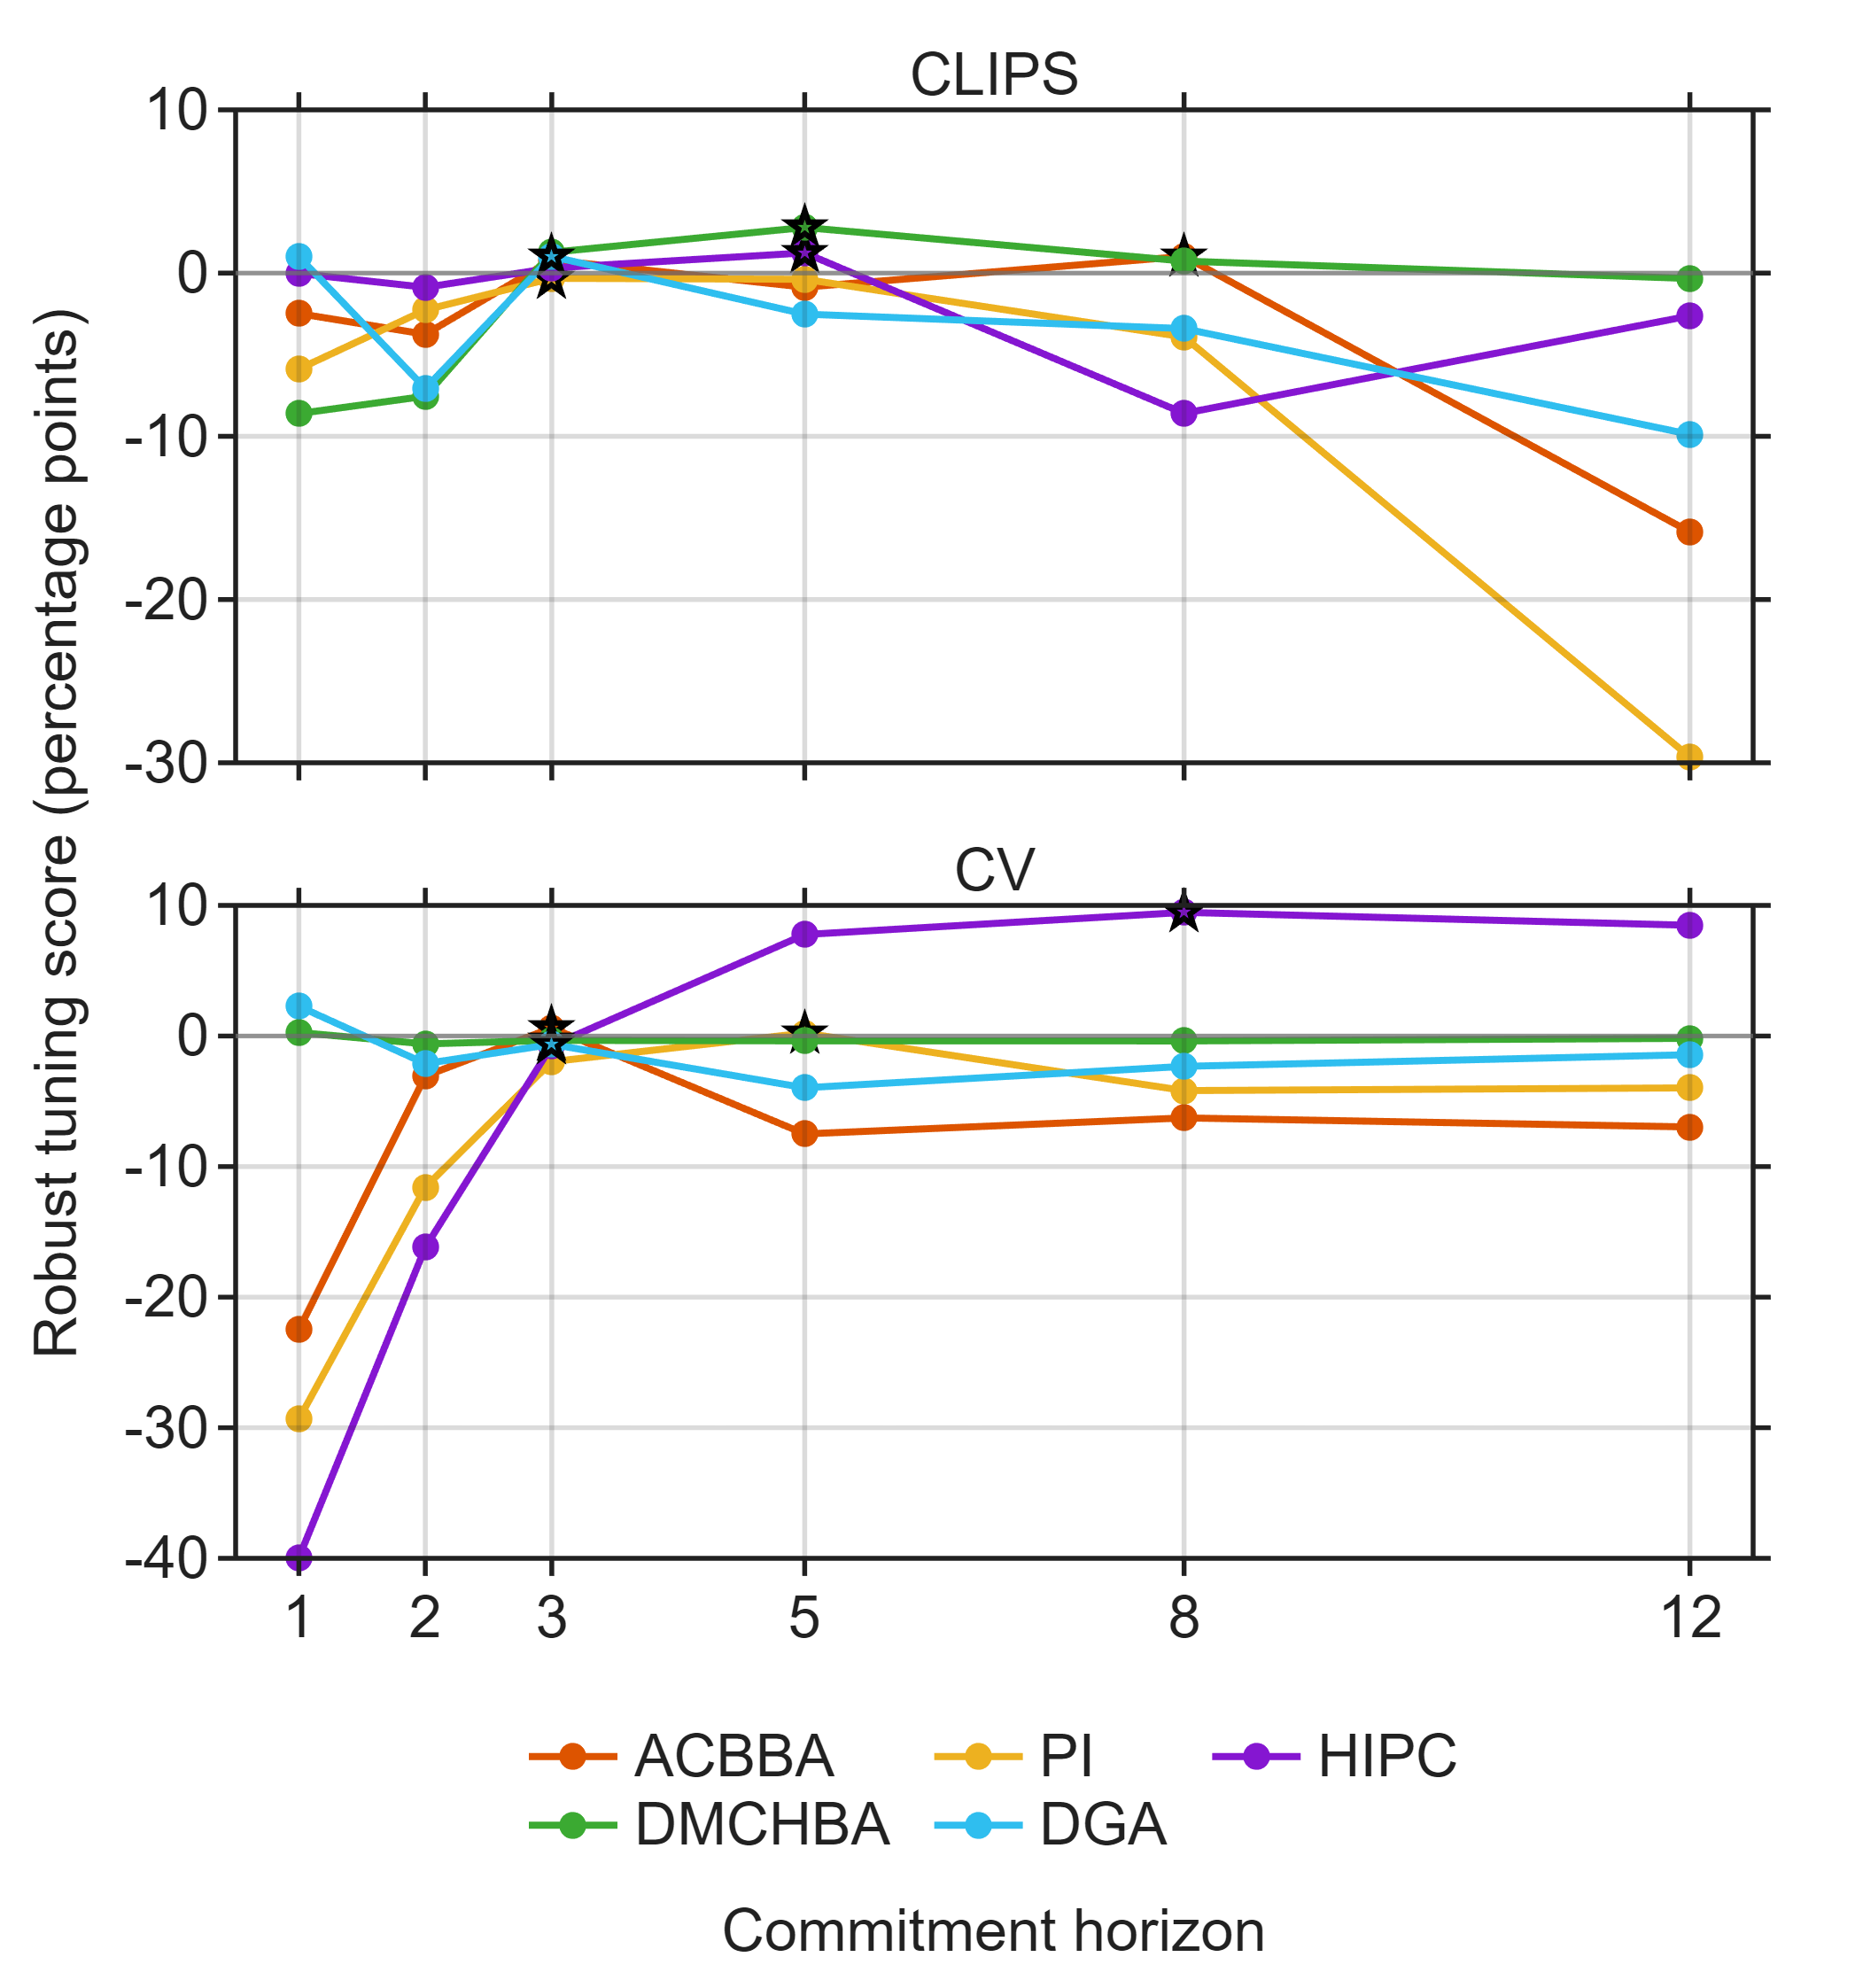
\includegraphics[width=\columnwidth]{figures/horizon_tuning.png}
    \caption{Commitment-horizon robust scores for CLIPS and CV. Higher scores indicate a more favorable balance of average improvement, communication-condition agreement, bad-condition performance, and local stability. Pentagrams mark the robust-score decision-table selections.}
    \label{fig:horizon_sensitivity}
\end{figure}
